%! TEX root = ../main.tex
\documentclass[main]{subfiles}

\begin{document}
\chapter{実験4:代理モデル使用時の最適化}
    \section{目的}
    これまでの章で,長野市バス運行スケジュール最適化問題の高速化のために,
    Walsh関数による代理モデルを使用するために必要な要素を決定した.
    本章では,これらの情報を用いて,実際に最適化問題に代理モデルを導入し,高速化が達成できているか検証する.
    ここで,代理モデルを導入した最適化を行った時,どのような結果を得ることが出来れば,高速化が達成できたと言えるのかを確認する.
    図\ref{hv_plot_}は,先行研究でのバス利用率4.5\%の時の世代数ごとのHVを表す.これは図\ref{hv_plot}と同一である.
    
    \begin{figure}
        \centering
        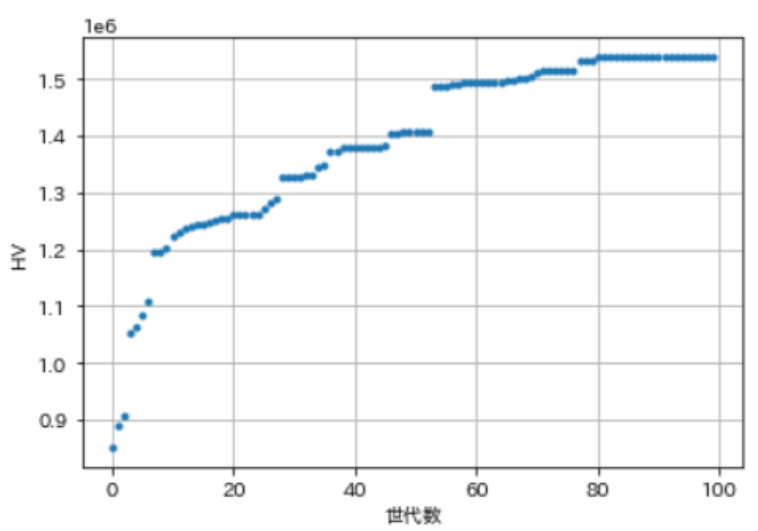
\includegraphics[width=\linewidth]{figures/hv_plot.png}
        \caption{バス利用率4.5\%の場合のHV推移}
        \label{hv_plot_}
    \end{figure}
    先行研究では100世代まで最適化を行い,そのHVが$1.538\times 10^6$であった.
    つまり,代理モデルを導入して最適化を行った結果,
    \begin{itemize}
        \item 100世代目のHVが$1.538\times 10^6$を超える
        \item 100世代目までにHVが$1.538\times 10^6$を超える
    \end{itemize}
    この2つのどちらかを満たしたとき,代理モデルによって最適化を高速化することが出来たと言える.
    
    また,先行研究で使用したアルゴリズムのフローチャートを図\ref{old_algo}に示す.
    \begin{figure}
        \centering
        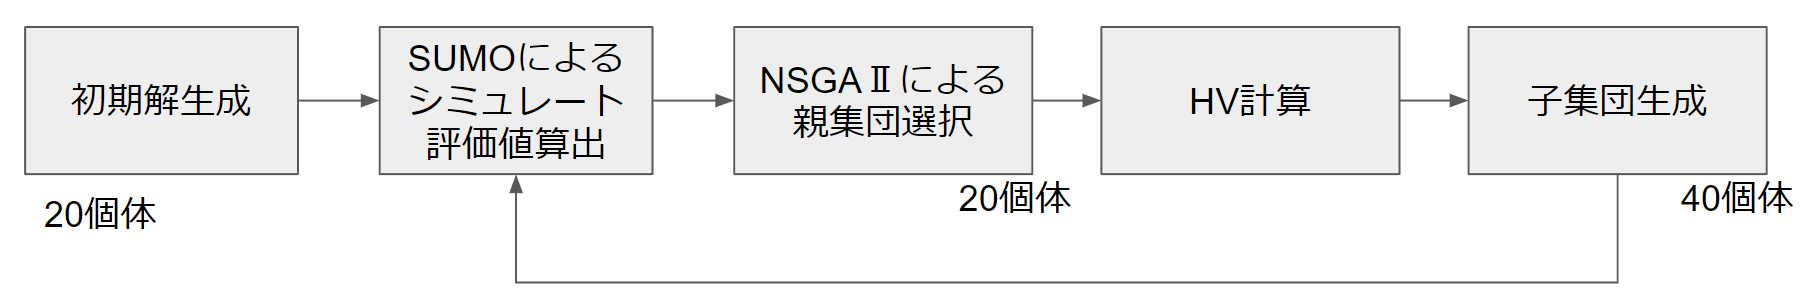
\includegraphics[width=\linewidth]{figures/old_algo.png}
        \caption{先行研究でのアルゴリズムのフローチャート}
        \label{old_algo}
    \end{figure}
    初期解を20個体生成させる.次に,HVを計算し,子集団を20個体生成する.
    新しい解である子集団20個体に対してSUMOによるシミュレートを行い評価値を算出する.
    親集団と子集団合わせた40個体に対し,NSGAⅡにより優れた解20個体を選択する.選ばれた20個体を親集団とする.
    このループを1世代として,ループを100回行うのが先行研究のアルゴリズムである.

    \section{実験方法}
    代理モデルの導入方法について2つの方法を検証した.
    以下でその2つについて,手法のフローチャートと特徴について述べる.
        \subsection{代理モデル内で進化型}
        図\ref{d}にフローチャートを示す.
        \begin{figure}
            \centering
            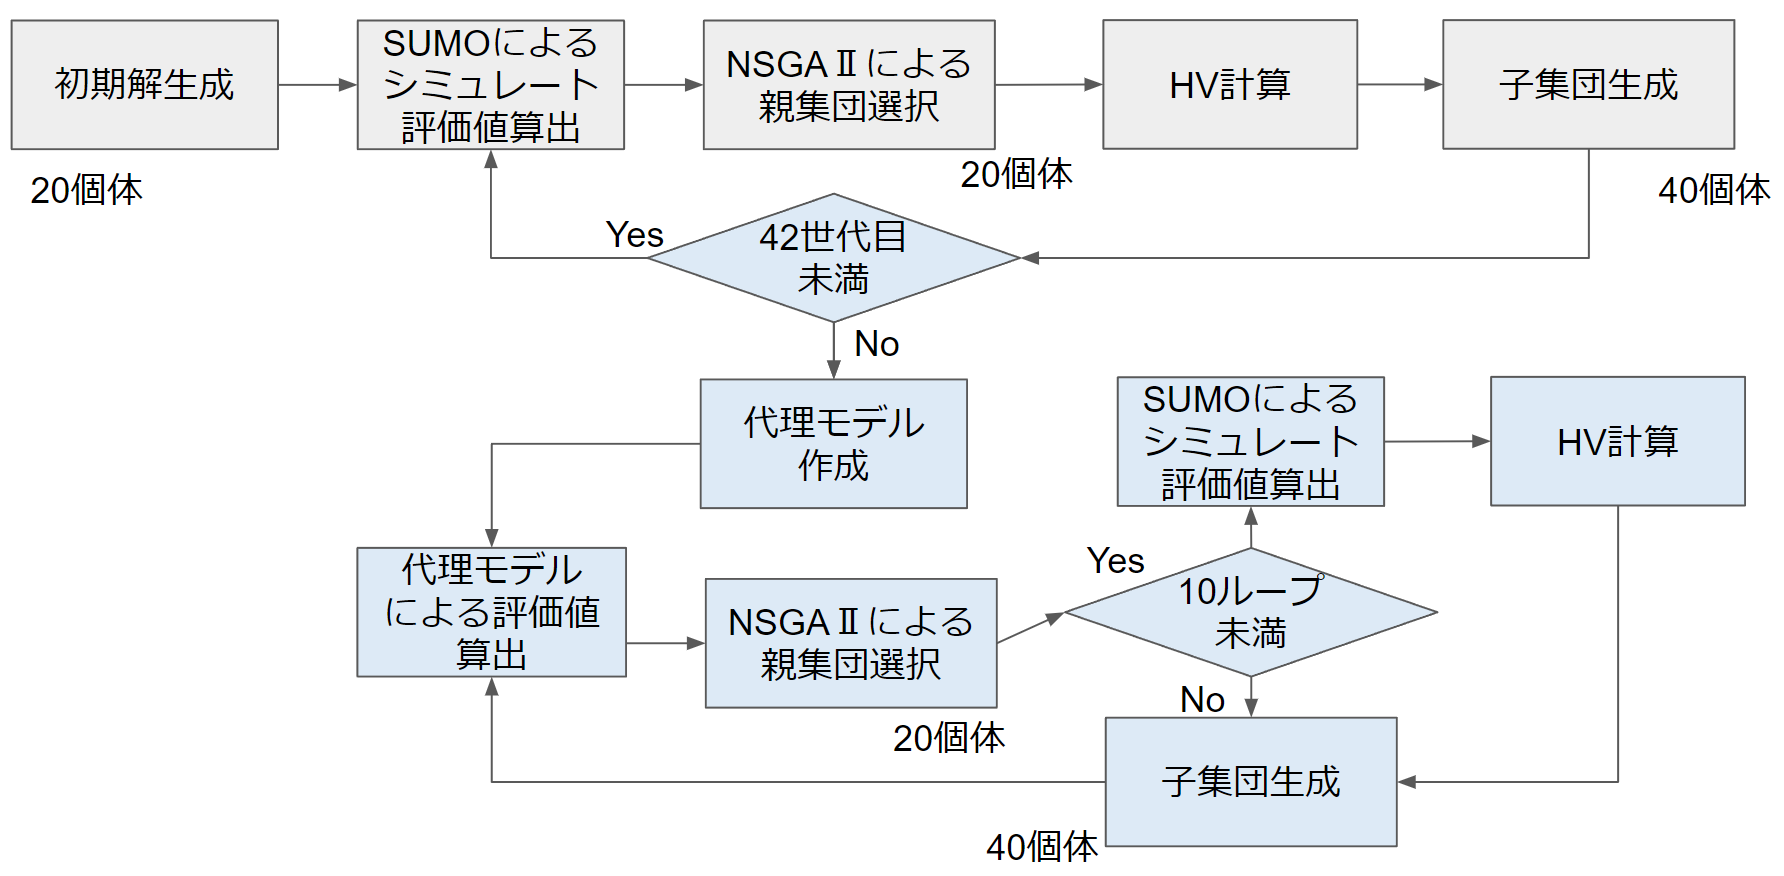
\includegraphics[width=\linewidth]{figures/d.png}
            \caption{代理モデル内で進化型}
            \label{d}
        \end{figure}



\end{document}